\section{Introduction}

The goal of the 3D spherical kernel is to offer to the user a large
set of functionalities on spheres, circles and circular arcs, in the 3D
space or restricted on a given sphere. These functionalities require 
computing on algebraic numbers,
which motivates the creation of a new kernel concept extending the
\cgal\ \ccc{Kernel} concept, that is restricted to objects
and functionality in a \ccc{FieldNumberType}.

All the choices (interface, robustness, representation, and so on)
made here are consistent with the choices made in the \cgal\ kernel,
for which we refer the user to the kernel manual
(Chapter~\ref{chapter-kernel-23}).

\section{Spherical Kernel Objects\label{section-SK-objects}}

New main geometric objects are introduced by \ccc{Spherical_kernel_3}:
circular arcs ((model of \ccc{SphericalKernel::CircularArc_3}), points
of circular arcs (model of \ccc{SphericalKernel::CircularArcPoint_3}),
and line segments (model of \ccc{SphericalKernel::LineArc_3}) whose
endpoints are points of this new type.

\ccc{SphericalKernel::CircularArcPoint_3} is used in particular for
endpoints of arcs and intersection points between spheres, circles or
arcs. The coordinates of these points are algebraic numbers of degree
two. Therefore, general predicates offered by the \ccc{Kernel} on
\ccc{Point_3}, which have coordinates in a \ccc{FieldNumberType},
would require heavy algebraic computations in algebraic extensions
of higher degrees and thus are not provided on
them, which explains the need for a new point type. 

A consistent set of predicates and constructions is offered on these
new types. 

\paragraph{General functionalities}~

The spherical kernel currently implements a set of
fundamental functionalities like intersection, comparisons, inclusion,
etc. More might be provided in the future, as long as only algebraic
numbers of degree two are used.

\paragraph{Functionalities relative to a sphere}~

%\label{section-def-on-sphere}
The interface of the underlying objects is extended by providing
additional operations that make sense only if the objects are
considered on the same sphere. For example, the result of the comparison of the
cylindrical or spherical coordinates of two points is well-defined
only when looking at them on a given common sphere. The presentation
of these operations requires the following definitions:

\textit{Coordinate system.}
Let consider a sphere with center \ccc{c} and radius \ccc{r}. Using
the Cartesian frame centered at \ccc{c}, we define a cylindrical
coordinate system $(\theta,z)$ on that sphere, with $\theta \in \left[
  0,2\pi \right)$ and $z \in \left[ -r,r \right]$. $\theta$ is given
in radian and measured in the $xy$-plane around the $z$-axis, starting
from $x>0$, $y=0$. The $z$-extremal points of a sphere are its North
and South poles defined as $(\theta,r)$ and $(\theta,-r)$
respectively, for any value of $\theta$. Observe that each point on
the sphere different from a pole corresponds to a unique pair
$(\theta,z)$.
% The poles of a sphere being its $z$-extremal points, we can observe
% that each point on a sphere different from a pole corresponds to a
% unique $(\theta,z)$ ( $(\theta,\pm r)$ define the same point for any
% value of $\theta$ ).  Note that the choice of a cylindrical
% coordinate system instead of spherical one comes from the fact that
% the comparison of $\phi$-coordinates is totally equivalent to the
% comparison of $z$-coordinates, and that $z$-coordinates are already
% used for the general objects in 3D.

\textit{Definition of a meridian.}
Given a sphere and its associated cylindrical coordinate system, a meridian of that
sphere is a circular arc consisting of the points having the same theta-coordinate
(the poles are the end points).
A plane containing the two poles of that sphere defines two meridians, one on each side
of the line passing through the poles. A vector $M$ whose direction is different from that of the latter
line defines a unique meridian on that sphere. The plane of that meridian is defined by the
direction of $M$ and the two poles. The sense of $M$ disambiguates the choice among the
pair of meridians thus defined.
On Fig.~\ref{fig-def-meridian}, the normal vectors $n_0$ and $n_1$ define 
two meridians of $S$: the circular arcs $A_0$ and $A_1$ respectively.

\begin{ccTexOnly}
\begin{figure}[ht!]
\centerline{
 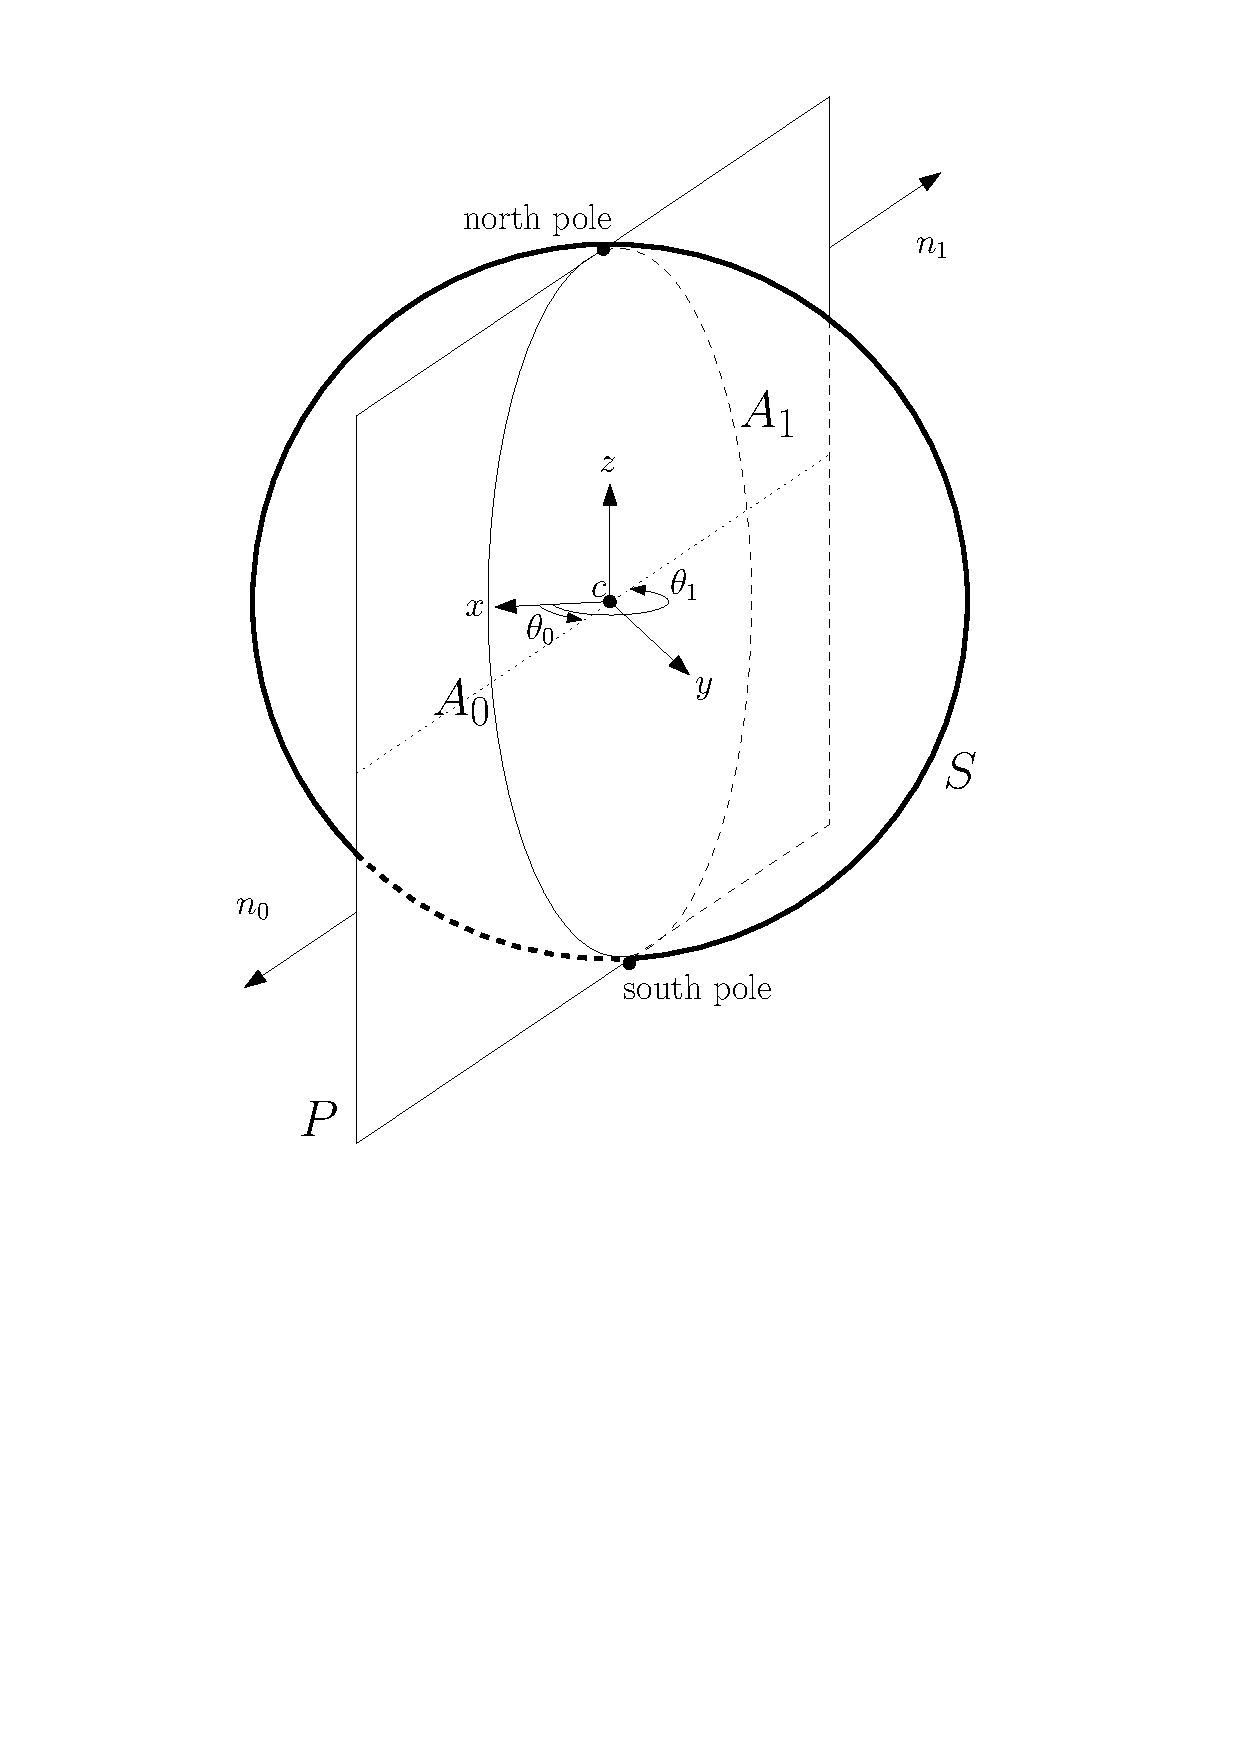
\includegraphics[height=.5\textwidth]{Circular_kernel_3/def_meridian}
}
\caption{Definition of two meridians on $S$, a sphere of center $c$.
The intersection of the plane $P$ (passing through the two poles of $S$)
and the sphere $S$ is a circle. The two poles of $S$ split that circle into two circular arcs $A_0$ and $A_1$, each being a meridian of $S$. 
The $\theta$-coordinates of meridians $A_0$ and $A_1$ are $\theta_0$ and $\theta_1= \theta_0 + \pi$ respectively.
\label{fig-def-meridian}}
\end{figure}
\end{ccTexOnly}

\begin{ccHtmlOnly}
  <CENTER>
    <img border=0 src="def_meridian.png" 
      alt="Definition of two meridians on $S$, a sphere of center $c$.
      The intersection of the plane $P$ (passing through the two poles of $S$)
      and the sphere $S$ is a circle. The two poles of $S$ split that circle
      into two circular arcs $A_0$ and $A_1$, each being a meridian of $S$. 
      The $\theta$-coordinates of meridians $A_0$ and $A_1$ are $\theta_0$
      and $\theta_1= \theta_0 + \pi$ respectively.">
  </CENTER>
\end{ccHtmlOnly}


\textit{Types of circles on a sphere.}
Given a sphere, a circle on that sphere is termed
\textit{polar} if it goes through only one pole, \textit{bipolar} if
it goes through the two poles of that sphere and \textit{threaded} if
it separates the sphere into two connected components, each
containing one pole. Any other circle is termed \textit{normal}. These
definitions are illustrated on Fig.~\ref{fig-def-circles}.

\begin{ccTexOnly}
\begin{figure}[ht!]
\centerline{
 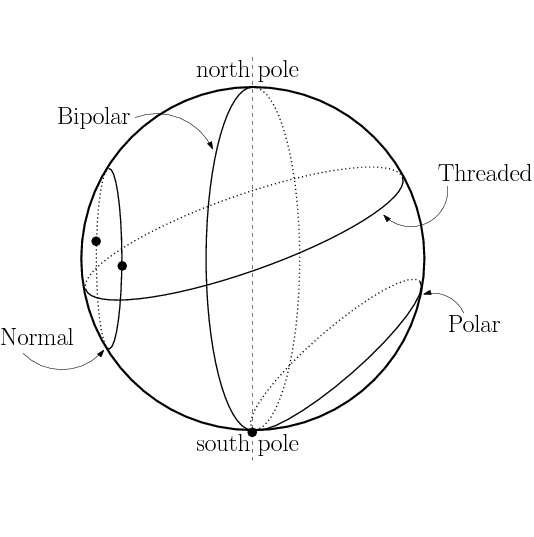
\includegraphics[height=.5\textwidth]{Circular_kernel_3/def_circles_extreme_pt}
}
\caption{The four types of circles on a sphere. Black dots
  are the $\theta$-extremal points.  \label{fig-def-circles}}
\end{figure}
\end{ccTexOnly}


\begin{ccHtmlOnly}
  <CENTER>
    <img border=0 src="def_circles_extreme_pt.png" 
      alt="The four types of circles on a sphere. Black dots are the
      $\theta$-extremal points."> 
  </CENTER>
\end{ccHtmlOnly}



% \begin{ccTexOnly}
% \begin{figure}[ht]
% \centerline{
%  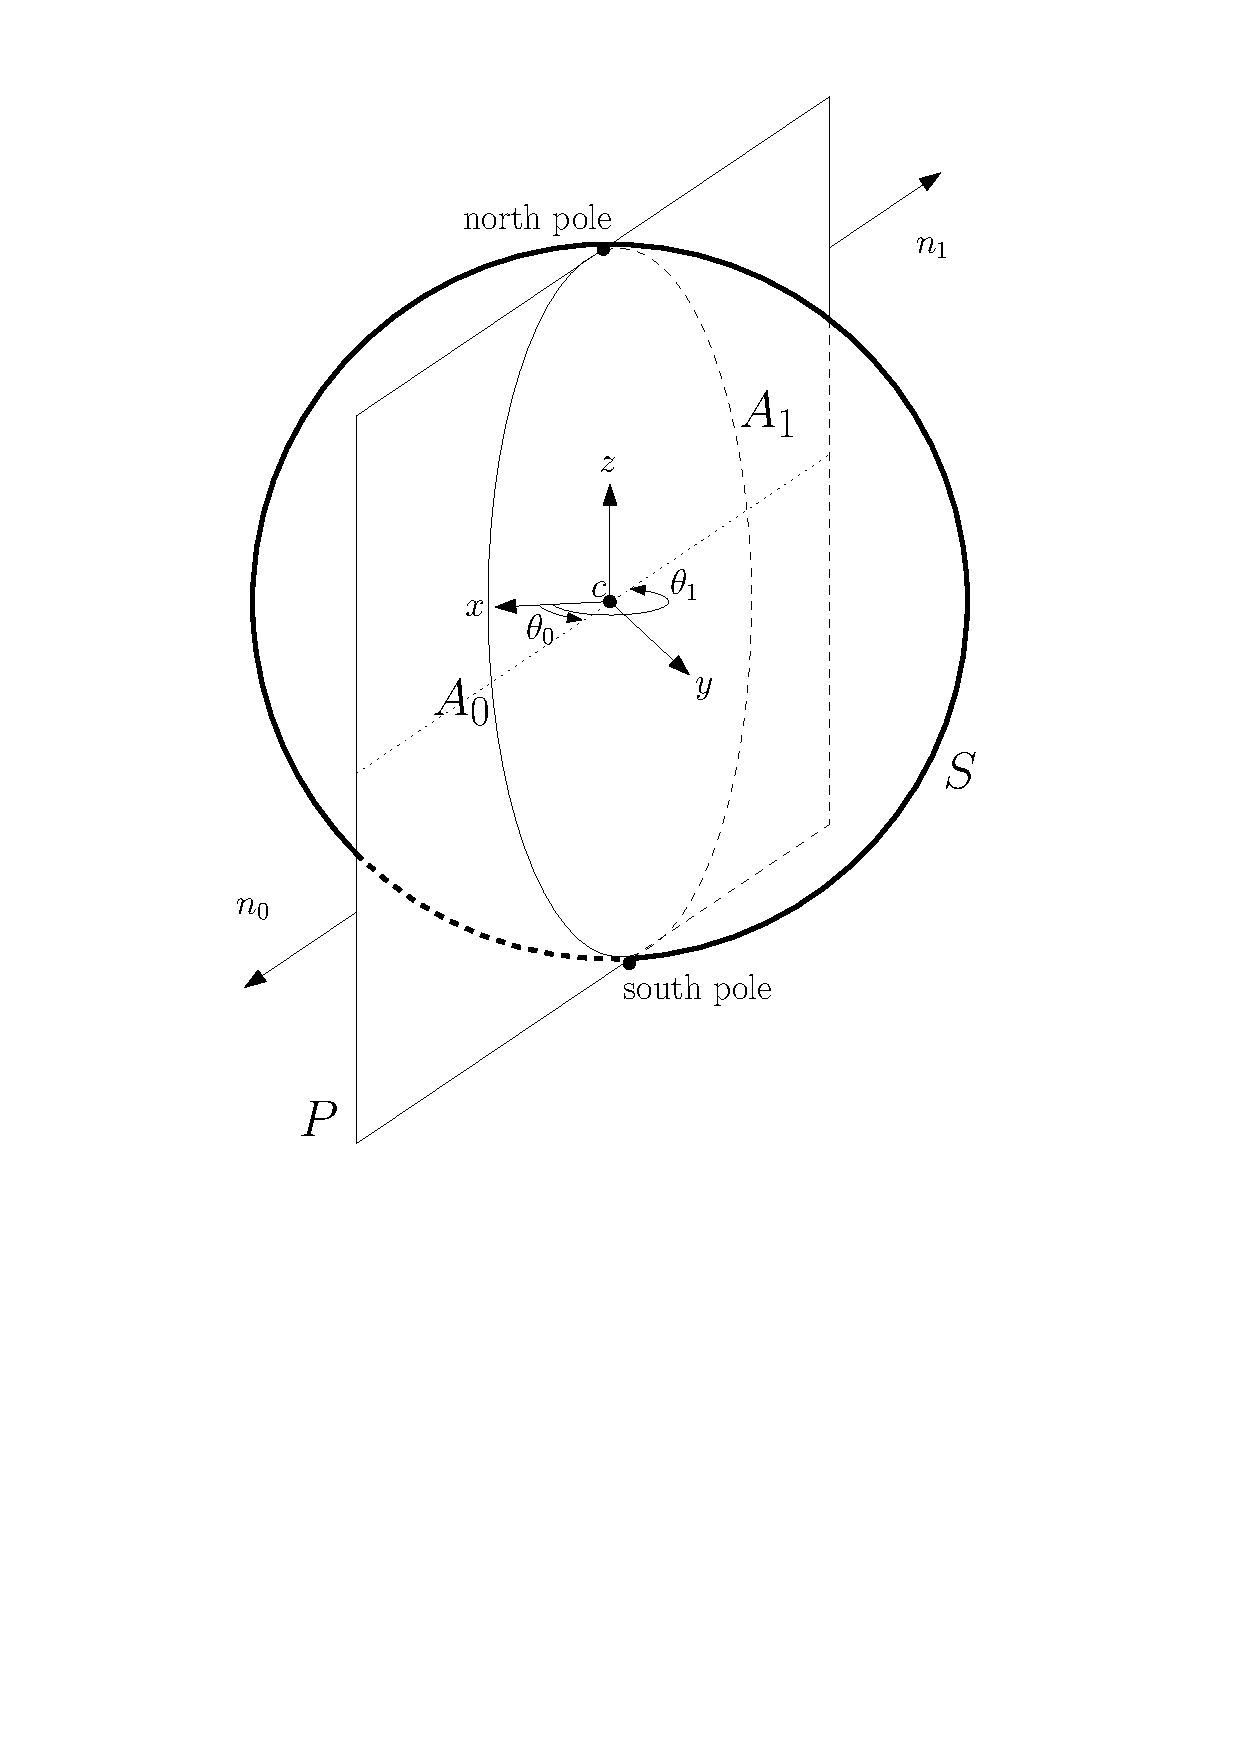
\includegraphics[height=.5\textwidth]{Circular_kernel_3/def_meridian}
% }
% \caption{Definition of a meridian. The intersection of the plane $P$ and the sphere $S$ is a circle.
% The two poles of $S$ split that circle into two circular arcs $A_0$ and $A_1$, each defining a meridian of $S$.
% \label{fig-def-meridian}}
% \end{figure} 
% \end{ccTexOnly}

% \begin{ccTexOnly}
% \begin{figure}[ht]
% \centerline{
%  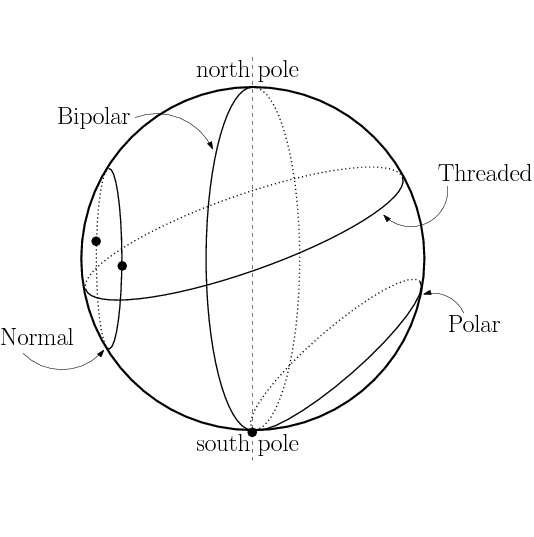
\includegraphics[height=.5\textwidth]{Circular_kernel_3/def_circles_extreme_pt}
% }
% \caption{The four types of circles on a sphere. Black dots
%   are the $\theta$-extremal points.  \label{fig-def-circles}}
% \end{figure} 
% \end{ccTexOnly} 

\textit{$\theta$-extremal points.}
Given a sphere one has:
a \textit{$\theta$-extremal point} of a normal circle is a point of
tangency between the circle and a meridian anchored at the poles of
that sphere.  Each normal circle defines two such points;
the $\theta$-extremal point of a polar circle is the pole the circle
goes through.  No such point is defined on a bipolar or a threaded
circle. 
These definitions are illustrated on Fig.~\ref{fig-def-circles}.
Notice that the $\theta$-extremal points should not be confused with
the endpoints of an arbitrary arc on a sphere.

The $\theta$-coordinate of a $\theta$-extremal point of a normal
circle on a sphere is well defined.
For a polar circle on a sphere, the plane containing the two poles and which is
tangent to that circle contains two different meridians. The
$\theta$-values of these meridians are the two $\theta$-coordinates
associated to the same $\theta$-extremal point of a polar circle.

\textit{$\theta$-monotone circular arcs.}
An arc on a sphere is said to be \textit{$\theta$-monotone} if any meridian
on that sphere intersects that arc in at most one point. With this definition, a
circular arc on a threaded circle is always $\theta$-monotone, and an
arc on a polar or normal circle is $\theta$-monotone if it does not
contain a $\theta$-extremal point, unless it is an endpoint. No such
arc is defined on a bipolar circle.

\section{Software Design}

The design of \ccc{Spherical_kernel_3} is similar to the design of
\ccc{Circular_kernel_2} (see Chapter~\ref{chapter-circular-kernel}). 
It has two template parameters:
\begin{itemize}
\item {} the first parameter must model the \cgal\ 
three dimensional \ccc{Kernel} concept. The spherical kernel derives
from it, and it provides all elementary geometric objects like points,
lines, spheres, circles and elementary functionality on them.
%The \cgal\ 2D Kernel can be used as parameter,
%but the user may plug his own kernel 
%instead, as long as it follows the \cgal\ kernel concept. 
\item {} the second parameter is the algebraic kernel, which is 
responsible for computations on polynomials and algebraic numbers. It 
must model the concept \ccc{AlgebraicKernelForSpheres}. The
robustness of the package relies on the fact that the algebraic kernel
provides exact computations on algebraic objects.
\end{itemize}

The 3D spherical kernel uses the extensibility scheme presented in the
kernel manual (see Section~\ref{section-extensible-kernel}). The types
of \ccc{Kernel} are inherited by the 3D spherical kernel and some
types are taken from the \ccc{AlgebraicKernelForSpheres}
parameter. \ccc{Spherical_kernel_3} introduces new geometric objects
as mentioned in Section~\ref{section-SK-objects}.

In fact, the spherical kernel is documented as a concept,
\ccc{SphericalKernel} and two models are provided: 
\begin{itemize}
\item {} \ccc{Spherical_kernel_3<Kernel,AlgebraicKernelForSpheres>}, the basic kernel,
\item {} and a predefined kernel \ccc{Exact_spherical_kernel_3}.
\end{itemize}

\section{Examples}

The first example shows how to construct spheres and compute
intersections on them using the global function.

\ccIncludeExampleCode{Circular_kernel_3/intersecting_spheres.cpp}

The second example illustrates the use of a functor. 

\ccIncludeExampleCode{Circular_kernel_3/functor_has_on_3.cpp}

  The third example illustrates the use of a functor on objects on the
  same sphere.  The intersection points of two circles on
  the same sphere are computed and their cylindrical coordinates are
  then compared.

\ccIncludeExampleCode{Circular_kernel_3/functor_compare_theta_3.cpp}

\section{Design and Implementation History}

This package follows the 2D circular kernel package (see
Chapter~\ref{chapter-circular-kernel}), which induced the basic
choices of design.

Julien Hazebrouck and Damien Leroy participated in a first
prototype.

  The first version of the package was co-authored by Pedro Machado
  Manh\~{a}es de Castro and Monique Teillaud, and integrated in CGAL
  3.4.  Fr\'ed\'eric Cazals and S\'ebastien Loriot extended the
  package by providing functionalities restricted on a given sphere
  \cite{cclt-dc3sk-08}.  

Sylvain Pion is acknowledged for helpful discussions.

This work was partially supported by the IST Programme of the 6th
Framework Programme of the EU as a STREP (FET Open Scheme) Project
under Contract No IST-006413 (\ccAnchor{http://acs.cs.rug.nl/}{ACS} -
Algorithms for Complex Shapes).
